% Для компиляции этого документа необходимо использовать движок XeLaTeX или LuaLaTeX
% и убедиться, что все шрифты поддерживают кириллические символы

\documentclass{article}
\usepackage[russian]{babel}
\usepackage{mathtools}
\usepackage{amsmath}
\usepackage{graphicx}
\usepackage{float}
\usepackage{hyperref}
\usepackage{units}
\usepackage{resizegather}
\DeclareMathOperator{\LPoi}{\text{LP}_{\text{01}}}
\DeclareMathOperator{\LPii}{\text{LP}_{\text{11}}}
\DeclareMathOperator{\im}{i}
\DeclareMathOperator{\e}{e}
\usepackage{commath}
\begin{document}
	
	\section{Экспериментальное подтверждение механизма МЧВС}
	
	Для подтверждения того, что процесс МЧВС на длине волны $1030~\text{нм}$ происходит в соответствии со схемой (\ref{eq:schemeIMFWM}), был проведён ряд экспериментов с лазерными импульсами на этой длине волны при отключённом сигнальном излучении на $1562~\text{нм}$. Были измерены спектры фундаментальной и высшей мод. Блок-схема экспериментальной установки представлена на рис.~\ref{fig:scheme_osa}.
	
	\begin{figure}[thbp]
		\centering
		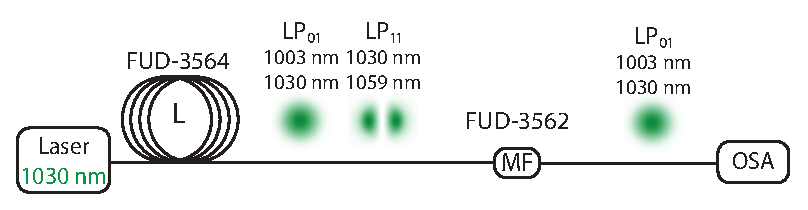
\includegraphics[width=0.99\linewidth]{images/imfwm/scheme_osa.eps}
		\caption{Экспериментальная установка для определения спектра моды $\LPii$. MF: модовый фильтр; OCA: анализатор спектра.}
		\label{fig:scheme_osa}
	\end{figure}
	
	Импульсы накачки на $1030~\text{нм}$ пропускались через волокно FUD-3564 длиной 4~м. Высшая мода $\LPii$ фильтровалась с помощью модового фильтра (МФ), состоящего из $10$-сантиметрового одномодового оптического волокна FUD-3562 \cite{fud3562} с модовым диаметром, близким к таковому у передающего волокна FUD-3564 в области $1~\text{мкм}$. Численное моделирование методом быстрого преобразования Фурье для распространения пучка (FFT-BPM) \cite{kawano2004introduction} показало, что после модового фильтра потери для мод $\LPoi$ и $\LPii$ в диапазоне длин волн $1000-1100~\text{нм}$ составили $2\%~(-0.09~\text{дБ})$ и $99\%~(-20~\text{дБ})$ соответственно.
	
	\begin{figure}[th]
		\centering
		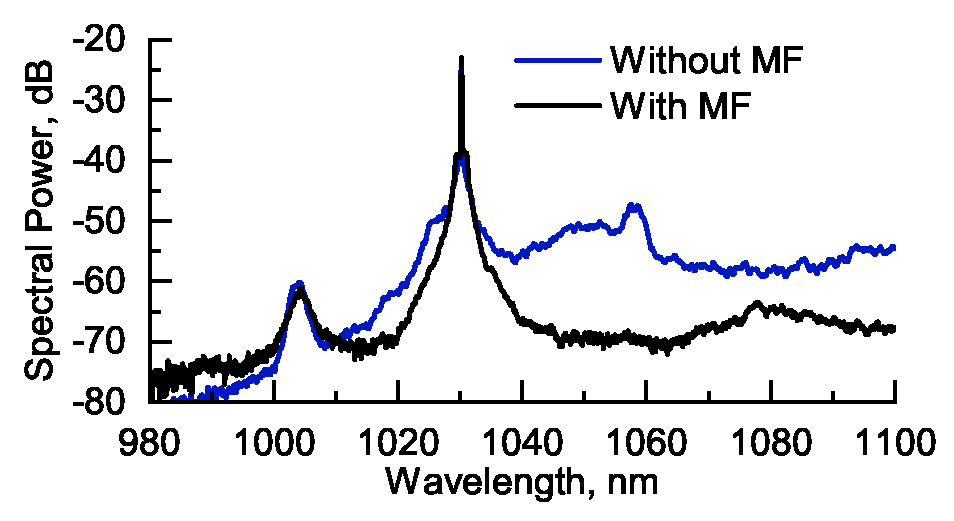
\includegraphics[width=0.7\linewidth]{images/imfwm/mode_filter_spectra.eps}
		\caption{Спектры в области $1~\text{мкм}$ с применением (чёрный) и без применения (синий) МФ.}
		\label{fig:mode_filter_spectra}
	\end{figure}
	
	Синяя и чёрная кривые на рис.~\ref{fig:mode_filter_spectra} представляют выходные спектры с применением и без применения МФ соответственно. Спектры демонстрируют минимальные различия (менее $0.5~\text{дБ}$) в областях $1030~\text{нм}$ (накачка) и $1003~\text{нм}$ (антистоксова компонента), что указывает на сохранение этих компонент. Однако в области около $1059~\text{нм}$ (стоксова компонента) применение МФ привело к существенному ослаблению на $20~\text{дБ}$. Это свидетельствует о присутствии моды $\LPii$ в данной спектральной области.
	
	\begin{figure}[th]
		\centering
		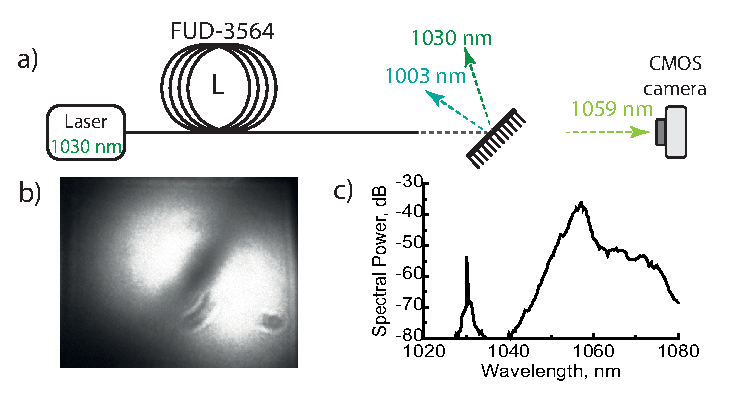
\includegraphics[width=0.9\linewidth]{images/imfwm/scheme_mirror.eps}
		\caption{a) Экспериментальная установка для визуализации пучка вблизи $1059$~нм; b) изображение пучка вблизи $1059$~нм; c) спектр после дихроичного фильтра.}
		\label{fig:scheme_mirror_lp11_spectra}
	\end{figure}
	
	Рис.~\ref{fig:scheme_mirror_lp11_spectra} a) показывает экспериментальную установку, использованную для визуализации пучка на длине волны $1059~\text{нм}$. Использовался дихроичный фильтр с высоким пропусканием $\left(\text{HT}>98~\%\right)$ в диапазоне $1050-1070~\text{нм}$ и высоким отражением $\left(\text{HR}>99~\%\right)$ в диапазоне $1000-1040~\text{нм}$. Изображение пучка (рис.~\ref{fig:scheme_mirror_lp11_spectra} b)) показывает, что значительная часть оптической мощности сосредоточена в моде $\LPii$ вблизи $1059~\text{нм}$ (рис.~\ref{fig:scheme_mirror_lp11_spectra} c)).
	
	Проведённые эксперименты подтверждают, что для импульсов накачки на $1030~\text{нм}$ процесс МЧВС происходит так, как указано в схеме (\ref{eq:schemeIMFWM}).
	
	Блок-схема экспериментальной установки для исследования взаимного влияния ММЧВС и ОМЧВС показана на рис.~\ref{fig:scheme_power}. Была измерена доля оптической мощности моды $\LPii$ в диапазоне $1000-1059~\text{нм}$ для случаев как синхронизированных, так и несинхронизированных импульсов накачки и сигнала. Соответствующие зависимости от длины передающего волокна $L$ показаны на рис.~\ref{fig:LP11Gain}.
	
	\begin{figure}[thbp]
		\centering
		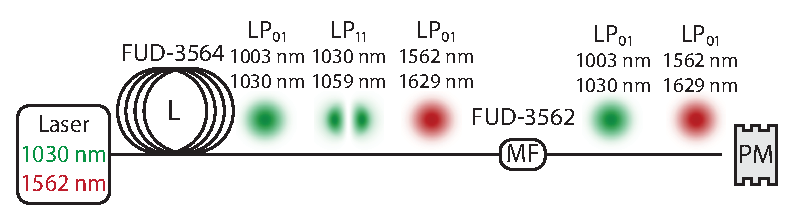
\includegraphics[width=0.95\linewidth]{images/imfwm/scheme_power.eps}
		\caption{Экспериментальная установка для измерения доли оптической мощности моды $\LPii$. МФ: модовый фильтр; ИМ: измеритель мощности.}
		\label{fig:scheme_power}
	\end{figure}
	
	Пиковые мощности импульсов накачки и сигнала составляли $5~\text{кВт}$ и $0.5~\text{кВт}$ соответственно. Чёрные и красные точки обозначают несинхронизированные и синхронизованные импульсы на длинах волн 1030~нм и 1562~нм. Для фильтрации высшей моды использовался тот же МФ, что и в предыдущих экспериментах. Потери для моды $\LPoi$ вблизи $1562~\text{нм}$ составили около $2\%~(-0.09~\text{дБ})$.
	
	\begin{figure}[h]
		\centering
		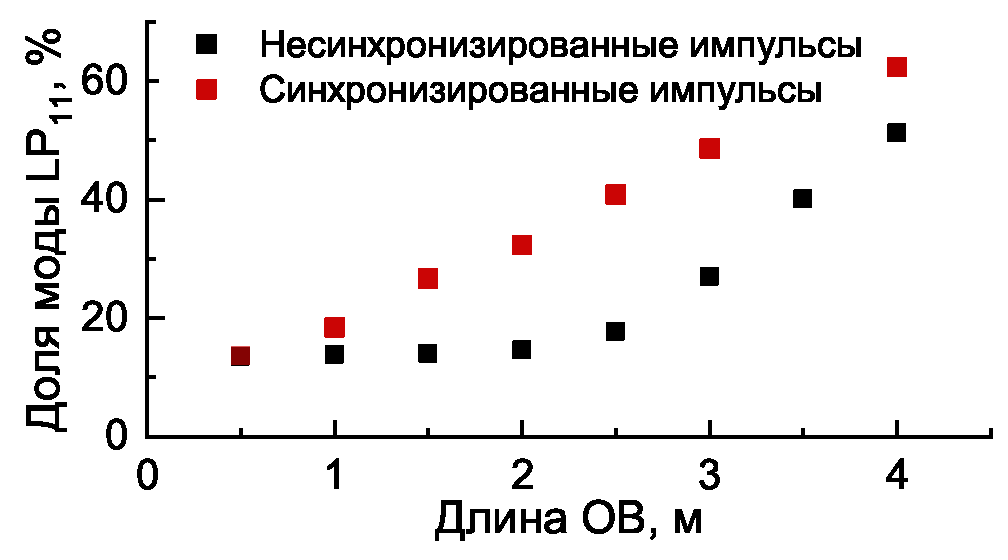
\includegraphics[width=0.65\linewidth]{images/imfwm/lp11Gain.eps}
		\caption{Зависимость доли мощности моды $\LPii$ в диапазоне длин волн $1000-1060~\text{нм}$ от длины передающего волокна для случаев несинхронизированных (чёрный) и синхронизированных (красный) импульсов накачки и сигнала.}
		\label{fig:LP11Gain}
	\end{figure}
	
	В случае малой длины передающего волокна $\left(L=0.5~\text{м}\right)$ нелинейные эффекты относительно слабы, и мода $\LPii$, распространяющаяся внутри волокна, присутствует преимущественно на длине волны $1030~\text{нм}$. Наличие моды $\LPii$ на этой длине волны на входе передающего волокна можно объяснить использованием маломодового активного волокна в схеме лазера. Дальнейшая синхронизация импульсов для длин передающего волокна $1 \leq L \leq 4~\text{м}$ приводит к росту доли мощности моды $\LPii$ вблизи $1059~\text{нм}$. Это свидетельствует о повышении эффективности процесса ММЧВС, происходящего в соответствии со схемой (\ref{eq:schemeIMFWM}), в случае синхронизированных импульсов.
	
	\section{Теоретическая модель}
	
	Нелинейно-оптические эффекты третьего порядка в оптических волокнах можно описать с помощью системы связанных нелинейных уравнений распространения \cite{agrawal2000nonlinear}:
	\begin{equation}
		\resizebox{0.99\textwidth}{!}{$%
			\left\{\begin{array}{@{}l@{}}
				\dfrac{dA_1}{dz}=\dfrac{\im n_{nl} \omega_1}{c}\!\left[\left(f_{11}\left|A_1\right|^2+\sum\limits_{k\neq1}f_{1k}\left|A_k\right|^2\right)\!A_1+2f_{1234}A_2^{\ast}A_3A_4\e^{\im \Delta k z}\right]\!, \vspace{0.05cm} \\ 
				\dfrac{dA_2}{dz}=\dfrac{\im n_{nl} \omega_2}{c}\!\left[\left(f_{22}\left|A_2\right|^2+\sum\limits_{k\neq2}f_{2k}\left|A_k\right|^2\right)\!A_2+2f_{2134}A_1^{\ast}A_3A_4\e^{\im \Delta k z}\right], \vspace{0.05cm} \\
				\dfrac{dA_3}{dz}=\dfrac{\im n_{nl} \omega_3}{c}\!\left[\left(f_{33}\left|A_3\right|^2+\sum\limits_{k\neq3}f_{3k}\left|A_k\right|^2\right)\!A_3+2f_{3412}A_4^{\ast}A_2A_1\e^{-\im \Delta k z}\right], \vspace{0.05cm} \\
				\dfrac{dA_4}{dz}=\dfrac{\im n_{nl} \omega_4}{c}\!\left[\left(f_{44}\left|A_4\right|^2+\sum\limits_{k\neq4}f_{4k}\left|A_k\right|^2\right)\!A_4+2f_{4312}A_3^{\ast}A_2A_1\e^{-\im \Delta k z}\right].
			\end{array}\right.\,$%
		}
		\label{eq:mainEQ}
	\end{equation}
	Здесь $A_{{i}}$~--- амплитуды взаимодействующих волн с циклическими частотами $\omega_i$; $n_{nl}$~--- нелинейный показатель преломления; $f_{ij}\text{ и }f_{ijkl}$ $\left(i,j,k,l\in\left[1,\,4\right]\right)$~--- интегралы перекрытия между поперечными модами оптического волокна и их парами соответственно; $z$~--- продольная координата; $\Delta k$~--- волновая расстройка:
	\begin{equation}
		\Delta k ={{n_3}\omega_3}/{c}+{{n_4}\omega_4}/{c}-{{n_1}\omega_1}/{c}-{{n_2}\omega_2}/{c}.
		\label{eq:deltaK}
	\end{equation}
	Здесь ${n_{i}}$~--- эффективный модовый индекс, $c$~--- скорость света в вакууме.
	
	В предположении, что эффективность ЧВС мала, можно записать следующее выражение для коэффициента параметрического усиления $g$ и эффективной волновой расстройки $\kappa$ для обоих процессов \cite{stolen1982parametric}:
	
	\begin{equation}
		g=\sqrt{\left(2\gamma\sqrt{P_1 P_2}\right)^2-\left(\kappa/2\right)^2}, \qquad 	\kappa = \Delta k + \gamma_1 P_1+\gamma_2 P_2,
		\label{eq:gainCoef}
	\end{equation}
	где $P_j=\abs{A_j\left(0\right)}^2$.
	
	В случае МЧВС, если считать, что длины волн близки $\left(\lambda^{\text{IM}}_{1,2}=1030~\text{нм}\right.$, $\left.\lambda^{\text{IM}}_3=1003~\text{нм}\right.$, $\left.\lambda^{\text{IM}}_4=1059~\text{нм}\right)$, и что модовые площади для одинаковых мод и их интегралы перекрытия совпадают:
	
	\begin{equation}
			\gamma_1^{\text{IM}}=\frac{n_{nl}\omega_1}{c A^{\text{eff}}_{\LPoi^{1030}}}, \quad
			\gamma_2^{\text{IM}}=\frac{n_{nl}\omega_1}{c A^{\text{eff}}_{\LPii^{1030}}}, \quad
			\gamma^{\text{IM}}=\frac{n_{nl}\omega_1}{c}f^{\text{IM}}_{3412}.
	\end{equation}
	
	Для ОМЧВС $\left(\lambda_1^{\text{FM}}= 1030~\text{нм}\right.$, $\left.\lambda_2^{\text{OM}}=1562~\text{нм}\right.$, $\left.\lambda_3^{\text{OM}}=1003~\text{нм}\right.$, $\left.\lambda_4^{\text{OM}}=1629~\text{нм}\right)$:
	
	\begin{equation}
		\gamma_1^{\text{FM}}=\frac{n_{nl}\omega_1}{c A^{\text{eff}}_{\LPoi^{1030}}},\quad
		\gamma_2^{\text{FM}}=\frac{n_{nl}\omega_2}{c A^{\text{eff}}_{\LPoi^{1562}}},\quad
		\gamma^{\text{FM}}=\frac{n_{nl}\left(\omega_1+\omega_2\right)}{2c}f^{\text{FM}}_{3412}.
	\end{equation}
	
	Здесь $A^{\text{eff}}$~--- эффективная модовая площадь, нижние индексы обозначают номер моды и соответствующую длину волны в нм, $\omega_1$ и $\omega_2$ соответствуют длинам волн $1030~\text{нм}$ и $1562~\text{нм}$ соответственно. Интегралы перекрытия $f^{\text{IM}}_{3412}$ и $f^{\text{FM}}_{3412}$ представляют степень перекрытия между парами мод, как определено в \cite{stolen1982parametric}. Верхний индекс обозначает тип процесса: IM для ММЧВС и FM для ОМЧВС.
	
	Рассматривая антистоксовы компоненты как для ММЧВС (рис.~\ref{fig:phase_sync}, чёрный), так и для ОМЧВС (рис.~\ref{fig:phase_sync}, красный), были рассчитаны спектры усиления (рис.~\ref{fig:phase_sync}, затенённые области) и кривые волновой расстройки (рис.~\ref{fig:phase_sync}, сплошные линии) с использованием соотношений (\ref{eq:gainCoef}). Длины волн $\lambda^{\text{IM, FM}}_1$ и $\lambda^{\text{IM}}_2$ были равны $1030~\text{нм}$, $\lambda^{\text{FM}}_2$ была равна $1562~\text{нм}$. Значения $\lambda^{\text{IM, FM}}_3$ изменялись, а $\lambda^{\text{IM, FM}}_4$ определялись по закону сохранения энергии.
	
	\begin{figure}[h]
		\centering
		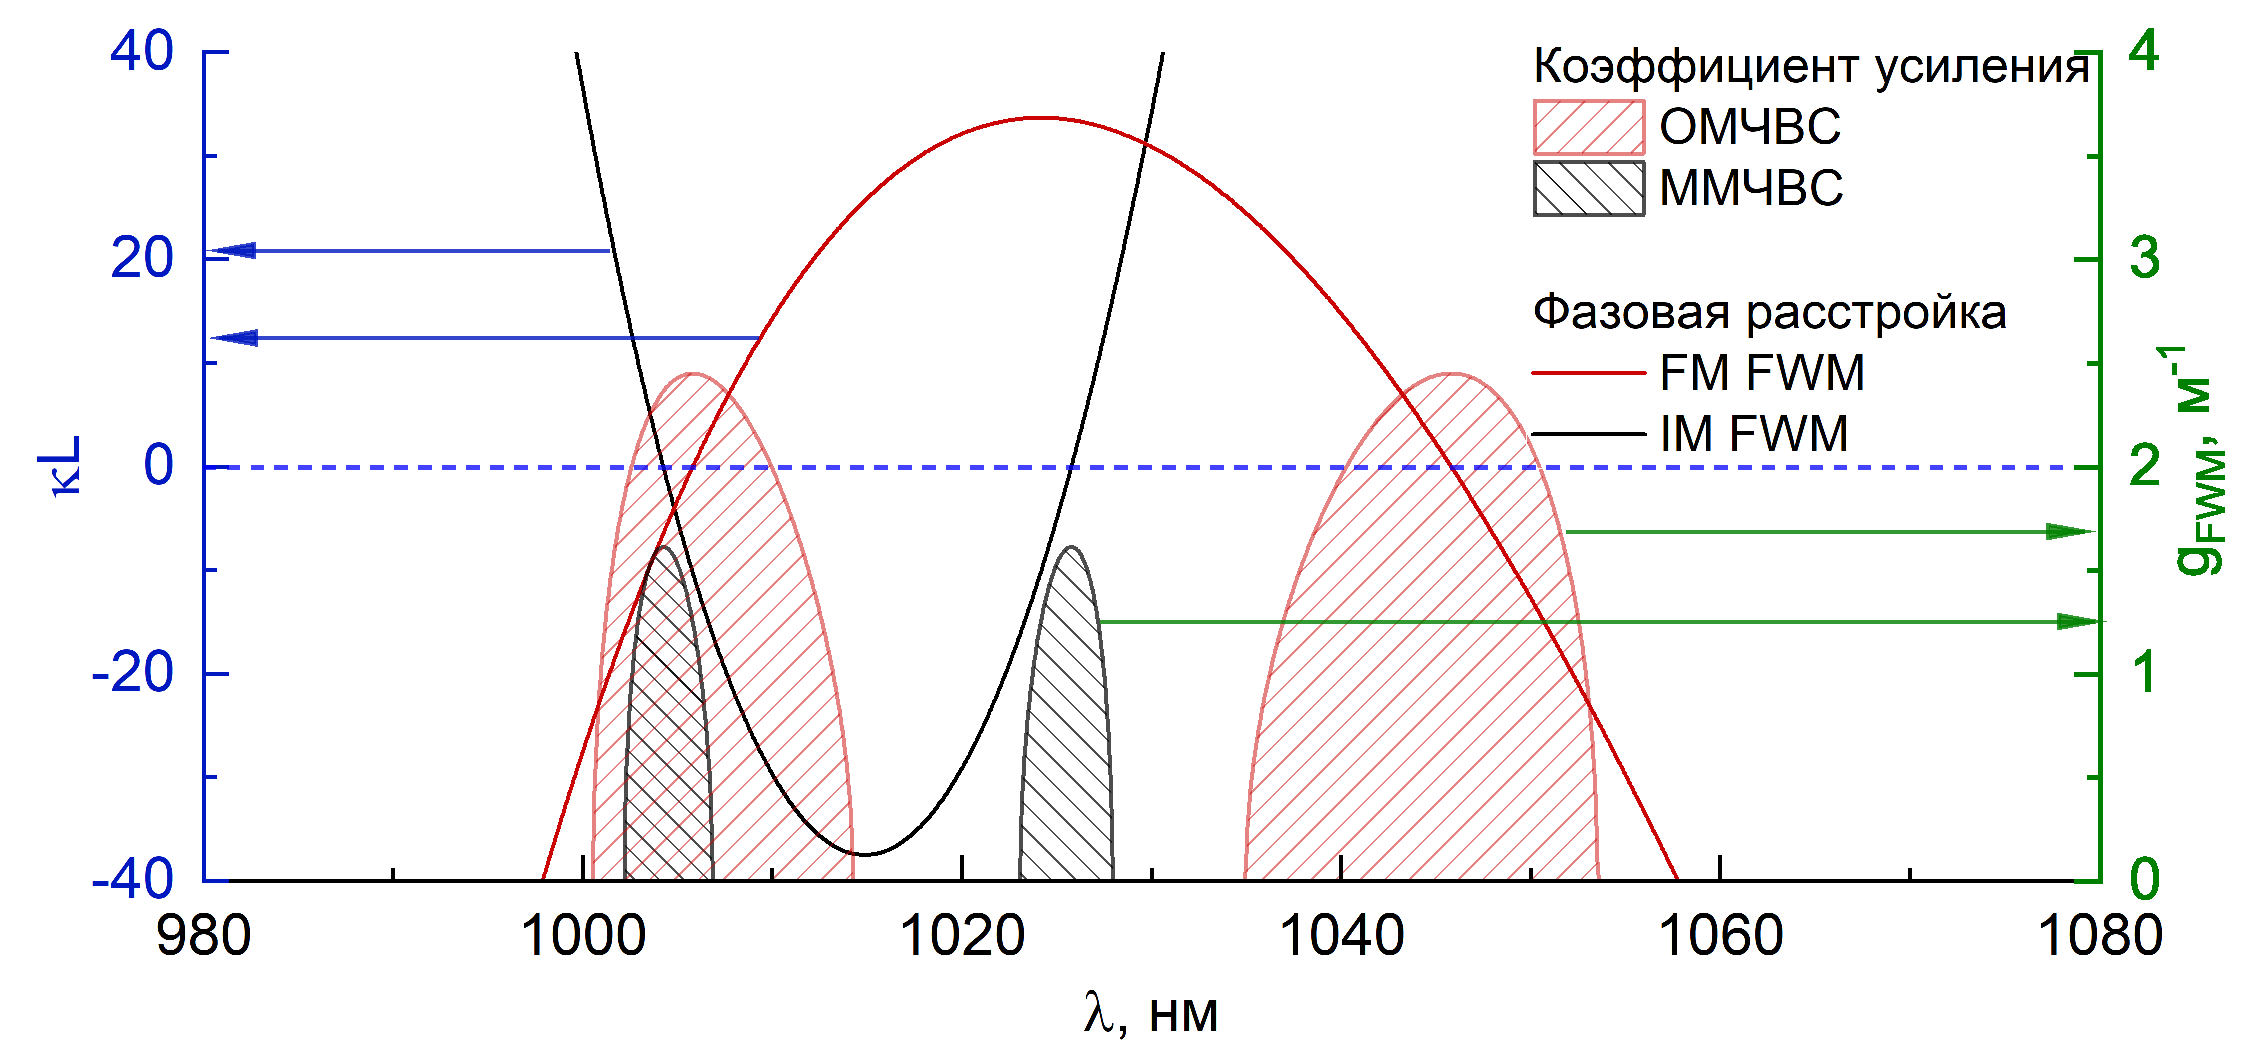
\includegraphics[width=0.85\linewidth]{images/imfwm/phase_sync_kappa.eps}
		\caption{Рассчитанная волновая расстройка (сплошные линии, левая шкала) и спектры усиления (затенённые области, правая шкала) для ОМЧВС (красный) и ММЧВС (чёрный). Длина передающего волокна: $L=4~\text{м}$.}
		\label{fig:phase_sync}
	\end{figure}
	
	Для обоих процессов ЧВС условие фазового синхронизма выполняется для антистоксовой компоненты вблизи длины волны $1003~\text{нм}$ в моде $\LPoi$. Это приводит к перекрытию спектров усиления ММЧВС и ОМЧВС вблизи этой длины волны. Поскольку амплитуда стоксовой компоненты пропорциональна амплитуде антистоксовой компоненты \cite{agrawal2000nonlinear}, наличие излучения на длине волны $1562$~нм приводит к увеличению мощности излучения моды $\LPii$ на $1059$~нм. Следует подчеркнуть, что для излучения в моде $\LPii$ на длине волны $1003~\text{нм}$ фазовый синхронизм отсутствует.
	
	Для моделирования распространения оптических импульсов в передающем волокне использовался метод BPM с конечными разностями (FD-BPM) \cite{kawano2004introduction}. Уравнения (\ref{eq:mainEQ}) решались численно. Значения максимальных пиковых мощностей накачки и сигнала, а также длина передающего волокна принимались равными $5.0~\text{кВт}$ на $1030~\text{нм}$, $0.5~\text{кВт}$ на $1562~\text{нм}$ и $L~=~4~\text{м}$ соответственно. Вследствие использования маломодового активного волокна в самом лазерном источнике доля моды $\LPii$ на входе передающего волокна предполагалась равной $15\%$ (см. рис.~\ref{fig:LP11Gain}). Нелинейный показатель преломления принимался равным $n_{nl}=2.5\cdot10^{-20}~\unitfrac{\text{Вт}}{\text{м}^2}$ \cite{agrawal2000nonlinear}.
	
	\begin{figure}[h]
		\centering
		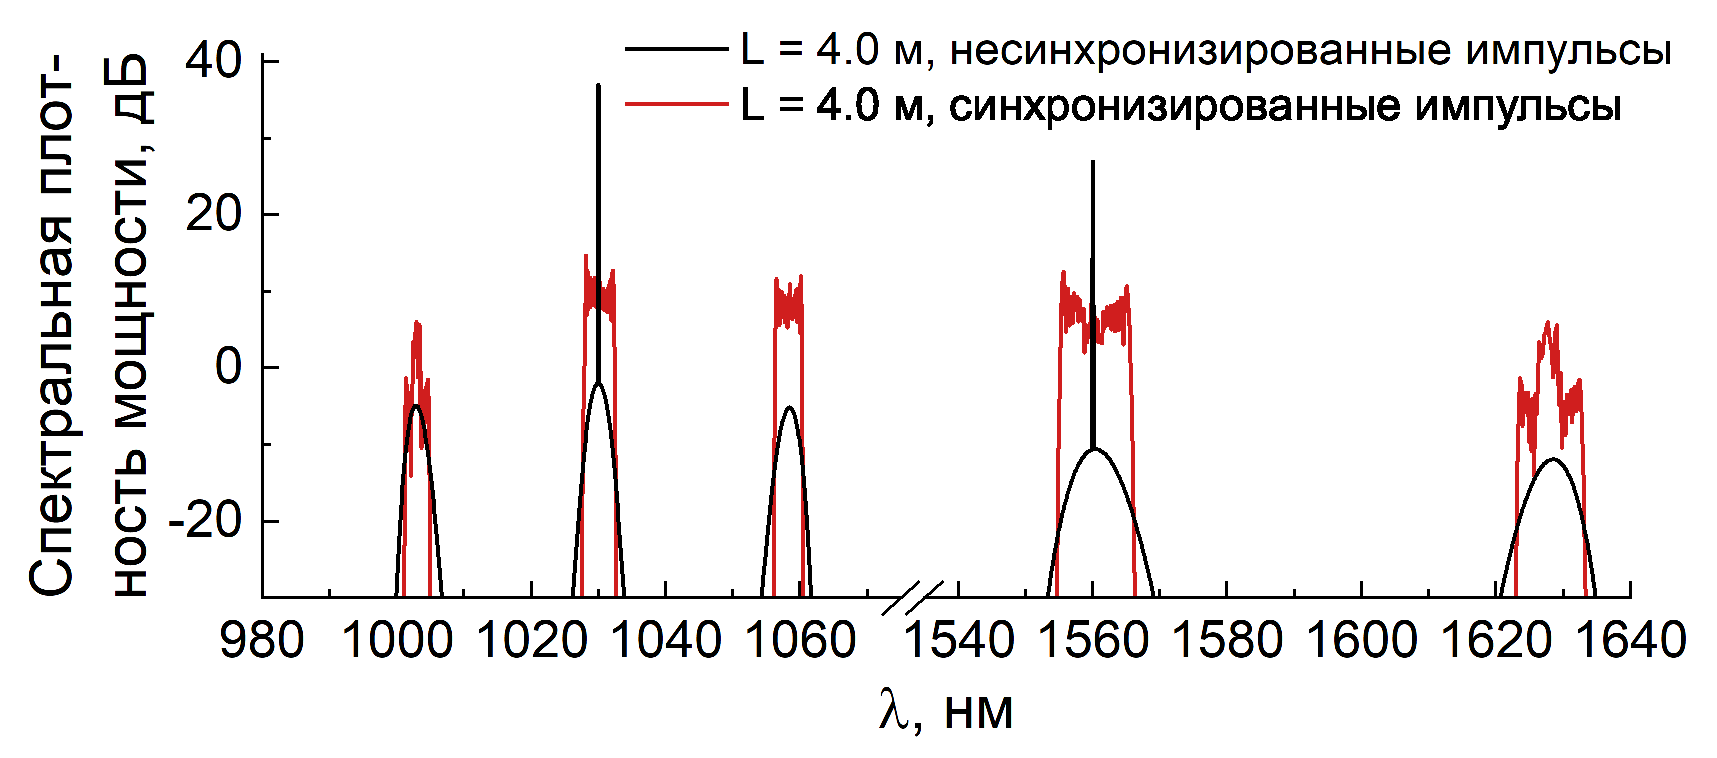
\includegraphics[width=0.9\linewidth]{images/imfwm/model_spectra.eps}
		\caption{Рассчитанные спектры двухволнового лазера для несинхронизированных (только ММЧВС, чёрный) и синхронизированных (ОМЧВС и ММЧВС, красный) импульсов.}
		\label{fig:model_spectra}
	\end{figure}
	
	Полученные результаты (см. рис.~\ref{fig:model_spectra}) показывают, что антистоксовы компоненты ОМЧВС и ММЧВС имеют близкие длины волн вблизи $1003~\text{нм}$, а также то, что взаимное влияние этих процессов ЧВС приводит к увеличению спектральной мощности соответствующих стоксовых и антистоксовых компонент до $20~\text{дБ}$.
	
	В итоге, наблюдаемый эффект увеличения эффективности МЧВС в случае синхронизированных импульсов накачки и сигнала подтверждён математическим моделированием.
	
	\section{Подавление МЧВС}
	
	Замена маломодового оптического волокна FUD-3564 на одномодовое волокно FUD-3562 в рассматриваемой лазерной схеме непрактична из-за высоких изгибных потерь этого волокна вблизи длины волны $1.5~\text{мкм}$. Использование многомодовых передающих волокон может помочь подавить нежелательные нелинейные эффекты. Однако применение волокон с большими сердцевинами неизбежно приводит к ухудшению качества выходного пучка $(M^2)$. В нашем случае существовали строгие требования к значению качества пучка для итогового $3~\text{мкм}$ лазерного источника, а именнно, $M^2 < 1.05$. В качестве альтернативы потенциально продуктивным является применение использованного МФ на входе передающего волокна. Такая реализация должна эффективно снизить долю моды $\LPii$ на входе передающего волокна с $15\%$ до менее чем $0.4\%$, тем самым повышая порог взаимного влияния процессов ЧВС. Нежелательный эффект уменьшения мощности моды накачки $\LPoi$ в диапазоне длин волн $1030.0\pm0.5~\text{нм}$ был бы смягчён, что привело бы к повышению эффективности генерации разностной частоты при сохранении требуемой длины передающего волокна.
	
	Зависимость от длины передающего волокна доли $\alpha$ оптической мощности моды $\LPoi$ в диапазоне длин волн $1030.0\pm0.5~\text{нм}$ рассчитывалась с использованием следующего выражения:
	\begin{equation}
		\alpha = \dfrac{\int_{1029.5~\text{нм}}^{1030.5~\text{нм}}{I\left(\lambda\right)d\lambda}}{ \int_{980~\text{нм}}^{1100~\text{нм}}{I\left(\lambda\right)d\lambda}}
		\label{eq:alpha}
	\end{equation}
	Здесь $I\left(\lambda\right)$ обозначает спектральную оптическую мощность на данной длине волны $\lambda$. Результаты применения МФ на входе передающего волокна показаны на рис. \ref{fig:suppression_with_spectrum}:
	
	\begin{figure}[thbp]
		\centering
		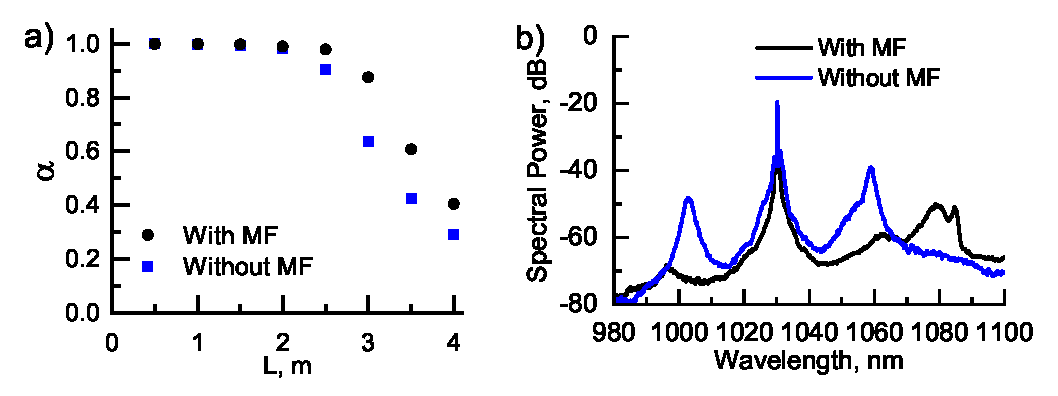
\includegraphics[width=0.99\linewidth]{images/imfwm/suppression_spectrum.eps}
		\caption{Зависимость доли оптической мощности $\alpha$ моды $\LPoi$ в диапазоне длин волн $1030.0\pm0.5~\text{нм}$ на выходе передающего волокна от его длины (a) и выходные спектры для длины передающего волокна $L=4~\text{м}$ (b) с применением и без применения МФ.}
		\label{fig:suppression_with_spectrum}
	\end{figure}
	Было получено, что для длины передающего волокна $L= 3~\text{м}$ применение МФ привело к уменьшению доли мощности моды $\LPii$ $\alpha$ на $30\%$ (см. рис. \ref{fig:suppression_with_spectrum} a)). Однако для длины передающего волокна $L= 4~\text{м}$ процессы ЧВС были подавлены, но усилилась стоксовая компонента ВКР, так что значение $\alpha$ было лишь на $15\%$ выше в случае применения МФ. На рис. \ref{fig:suppression_with_spectrum} b) видно, что без МФ ВКР подавлялось процессами ЧВС. Можно сделать вывод, что использование МФ позволяет удлинить передающее волокно до $0.5~\text{м}$ с незначительным влиянием на долю оптической мощности в диапазоне $1030.0\pm0.5~\text{нм}$.
	
	\section{Заключение}
	
	В данной главе впервые представлены результаты экспериментальных и численных исследований взаимного влияния ММЧВС и ОМЧВС. В частности, было изучено распространение наносекундных оптических импульсов на длинах волн $1030~\text{нм}$ и $1562~\text{нм}$ в маломодовом передающем волокне FUD-3564. Такое взаимное влияние накладывает серьёзные ограничения на максимальную длину передающего волокна двухволновой лазерной системы, а также на эффективность последующего процесса генерации разностной частоты. Взаимодействие между ММЧВС и ОМЧВС происходит из-за перекрытия спектров усиления их антистоксовых компонент. Для подавления этого эффекта предлагается установка МФ на входе передающего волокна, что позволяет увеличить допустимую длину передающего волокна до $0.5~\text{м}$ с пренебрежимо малым влиянием на мощность накачки в диапазоне $1030.0\pm0.5~\text{нм}$.
	
\end{document}